\documentclass[conference]{IEEEtran}
\IEEEoverridecommandlockouts
\usepackage{anyfontsize}
\usepackage{cite}
\usepackage{amsmath,amssymb,amsfonts}
\usepackage{algorithmic}
\usepackage{graphicx}
\usepackage{textcomp}
\usepackage{hyperref}
\usepackage{xcolor}
\usepackage{pgfgantt}

\begin{document}

\title{%
    Diffusion Models for Machine Learning \\
    \huge CS 584 Final Report}

\author{\IEEEauthorblockN{1\textsuperscript{st} Isaias Rivera}
    \IEEEauthorblockA{\textit{College of Computing} \\
        \textit{Illinois Institute of Technology}\\
        Chicago, Illinois, USA \\
        irivera3@hawk.iit.edu}
}

\maketitle

\section{Introduction}

\fontsize{14}{14}\selectfont

Diffusion models are a type of generative model that utilizes the principles of
diffusion to generate realistic data. There are different types of diffusion
models that have the same underlying idea including, diffusion probabilistic
models, noise-conditioned score network, and denoising diffusion probabilistic
models \cite{weng2021diffusion}.

The basic idea behind diffusion-based generative models is that noise is first
added to an initial input, where the resulting noisy image is then processed to
subsequently remove that noise, while preserving the underlying structure of
the image. This process is done multiple times where, at each step of this
process, the noise level is decreased, and the resulting image becomes more and
more refined. After this training, the model can then be used to generate data
by passing random noise through the learned denoising process.

Diffusion-based generative models can function either unconditionally or guided
such as with GLIDE's text-guided diffusion model, trading "diversity for
fidelity"\cite{GLIDE}. There are other examples of this online such as with
Google's Imagen, and OpenAI's DALL-E 2.

There are many
variations\cite{hoCF}\cite{kerasDDPM}\cite{pmlr-v162-nichol22a}\cite{hugimpl}
and different improvements\cite{nichol2021improved}\cite{song2022denoising} to
diffusion models that are being actively researched and have already been
implemented, however, as in my proposal I mainly have wanted to explore
implementing my own in an easily digestible format.

\section {Focus}

The main focus of my project has been with Denoising diffusion probabilistic
models, or DDPM for short, as I have found the most literature revolving around
this variation on diffusion models. I have not gone further than DDPMs,
however, there are plenty of different perspectives and variations on DDPMs
that have been made\cite{hugimpl}. Regardless, a good part of my research has
been with understanding both the math and implementation of every step with a
DDPM\cite{nain2022-2}\cite{nain2022-3}\cite{ho2020denoising}. However, the major component has been focused on compiling a very simple DDPM in jupyter that attempts to prevent delegating parts of the process off to an API, both to learn about the entire process and reach a point where images can be generated.

\section {Implementation}

The model that I have compiled consists of a very simple DDPM, with limited
complexity. This allows it to be easier to understand, however, it is also very
poor in terms of performance. My main notebook uses torch to implement
everything, however, I have found many implementations that use a variety of
APIs.

\subsection{The Forward Process}

The forward process is the step that involves adding noise to data. Given a
number of timesteps, gaussian noise is added to data at each step, where
subsequent steps are dependent on the output of the previous step. The main
equation that describes this, is as follows

$$
    q(x_{1:T}\vert x_{0})
    := \prod_{t=1}^{T}q(x_{t}\vert x_{t-1})
$$

$$
    :=\prod_{t=1}^{T}\mathcal{N}(x_{t};\sqrt{1-\beta_{t}} x_{t-1},\ \beta_{t}\bf I)
$$

Where $T$ is the total number of timesteps, $\beta_t$ is the variance schedule,
where $\beta_t \in (0,1)$ and $\beta_{1} < \beta_{2}...$, it describes the
amount of noise we want to add to each timestep. This schedule can simply be
set as linear, however, a cosine schedule has been proven to improve the
performance of the model\cite{nichol2021improved} as it smooths out the rate at
which the data is destroyed. Figure \ref{fig:vsc} shows this.

\begin{figure}[htbp]
    \centering
    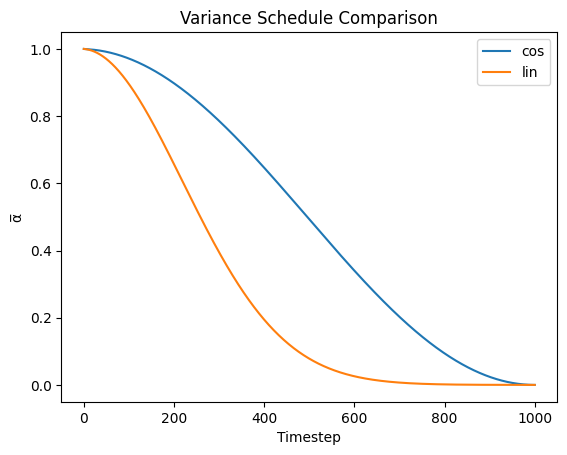
\includegraphics[width=0.45\textwidth]{../images/schedule.png}
    \caption{Variance Schedule Comparison}
    \label{fig:vsc}
\end{figure}

\subsubsection{Reparameterization}

Reparameterization of the forward process allows for the forward process to be
sampled at any given timestep. What this mainly involves is taking the fact
that, given two gaussian distributions, the sum these variables are the same as
the sum of their mean and variances $\mathcal{N}(\mu_{1} + \mu_{2},
    \sigma_{1}^2 +\sigma_{2}^2)$ \cite{nain2022-3}

What this allows us to do is,instead of just using the beta schedule as is, we
use $\bar{\alpha}$, where $\alpha_{t} = 1 - \beta_{t},$ and $\bar{\alpha}_{t} =
    \prod_{i=1}^T \alpha_{i}$

This speeds up the forward diffusion process, which is especially helpful, as
it is later randomly sampled in order to train the model.

\subsection{The Reverse Process}

The reverse process involves sampling the forward process using a random
timestep and predicting the noise in that sample. Where a neural network is
trained to predict this noise.

The following equation describes this process.

$$
    p_{\theta}(x_{0:T})
    := p(x_{T}) \prod_{t=1}^T p_{\theta}(x_{t-1} | x_{t})
$$

$$
    := p(x_{T}) \prod_{t=1}^T \mathcal{N}(x_{t-1}; \mu_{\theta}(x_{t}, t), \Sigma_{\theta}(x_{t}, t))
$$

Where $X_{t-1}$ is predicted using the current timestep.

\subsection{Timestep Embedding}

Timestep Embedding, or positional embedding, is used to ensure that the model
captures dynamics of the data over time. The original paper employs sinusoidal
position embeddings to encode $t$. This is achieved by adding an additional
channel to the input of each layer of a u-net. However, results are still
relatively similar when this embedding is placed within the first input, which
is what is done with the simple implementation.

\subsection{Loss Function}

The most common form of loss used is Huber loss, which is a hybrid of Huber
loss balances the strengths of Mean Squared Error and Mean Absolute Error
loss\cite{kerasDDPM}.

\subsection{U-Net}

A U-Net is a type of neural network architecture primarily in image
segmentation tasks. It consists of an encoder and a decoder network with skip
connections between them, which allows it to perform highly accurate
segmentation of objects in images with relatively few training examples. Figure
\ref{fig:unetarc}

\begin{figure}[htbp]
    \centering
    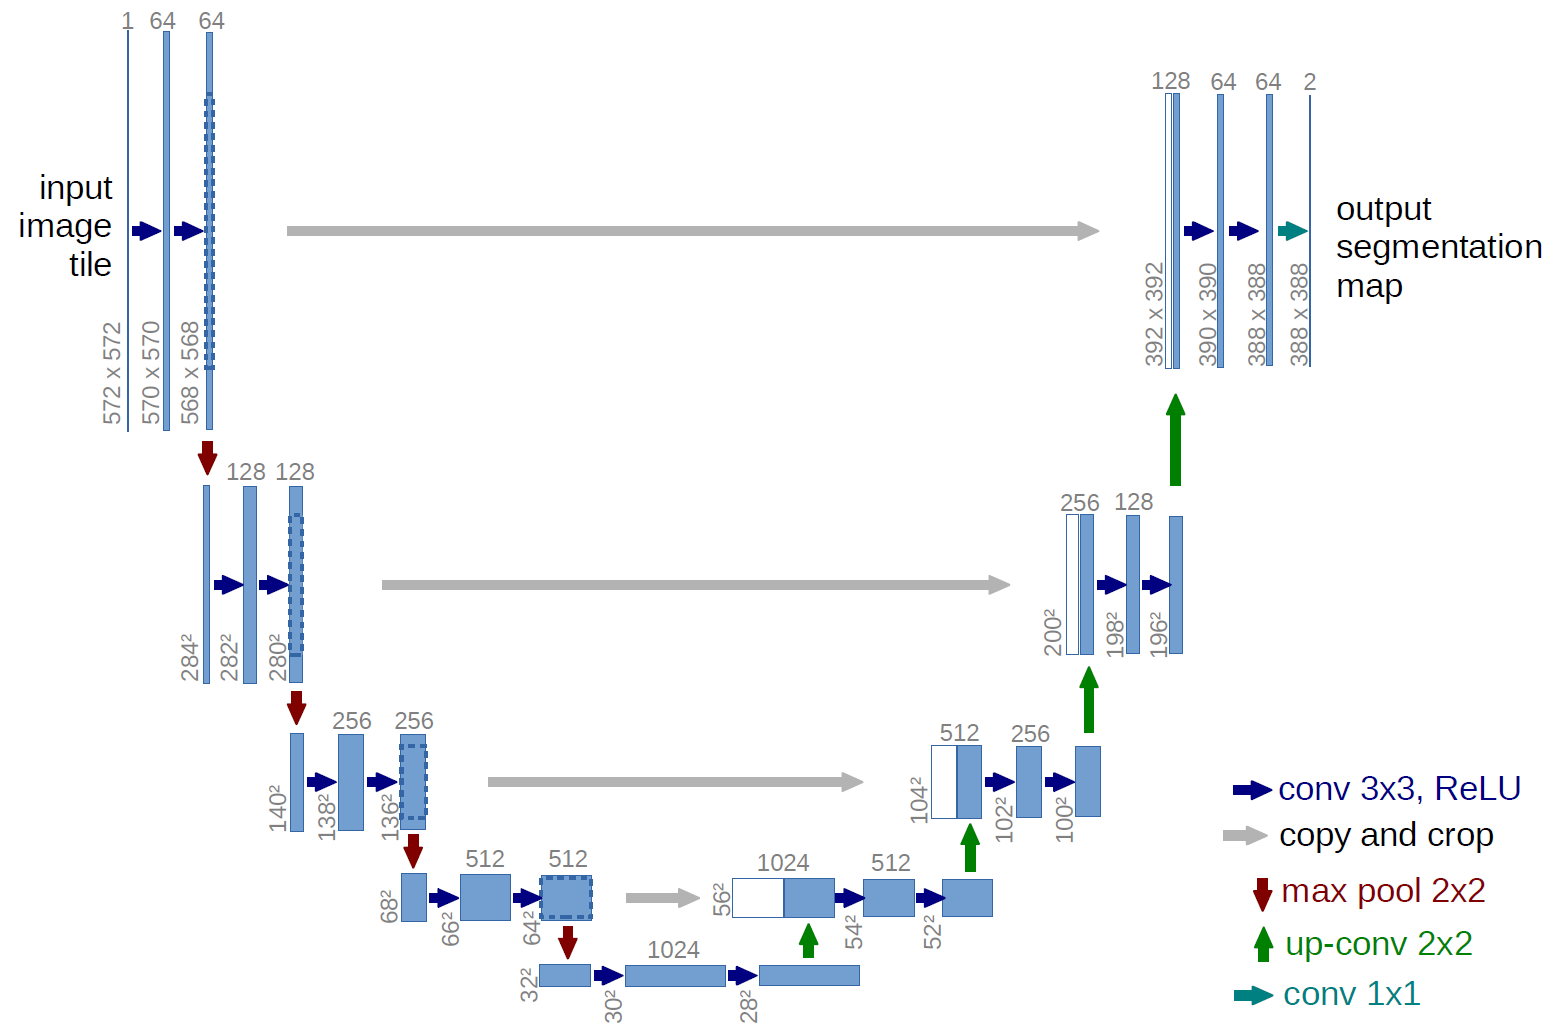
\includegraphics[width=0.45\textwidth]{../images/u-net-architecture.png}
    \caption{U-net architecture (example for 32x32 pixels in the lowest resolution). Each blue box corresponds to a multi-channel feature map. The number of channels is denoted on top of the box. The x-y-size is provided at the lower left edge of the box. White boxes represent copied feature maps. The arrows denote the different operations. \cite{RFB15a}}
    \label{fig:unetarc}
\end{figure}

A U-Net is the model used by the original DDPM paper, however, it is not the
only model that can be used. But for this example, I used a very simplified
version of the model\cite{AmanU-net} to aid in understanding the entire
process.

\subsection{Training}

\begin{figure}[htbp]
    \centering
    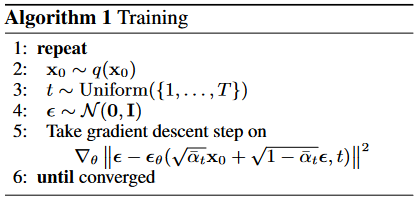
\includegraphics[width=0.45\textwidth]{../images/train.png}
    \caption{Training algorithm}
    \label{fig:Train}
\end{figure}

Figure \ref{fig:Train} is the training algorithm as described in the original
DDPM paper. However, simply put, we take a sample at a random timestep of the
forward diffusion process and use a model to learn the noise that is added on.
Additionally, it should be noted that, because this is typically done in
batches, something like stochastic gradient descent is in use to optimize
models. In the case of the simplified model, Adam is in use, as many
implementations default to using it.

\subsection{Sampling}

\begin{figure}[htbp]
    \centering
    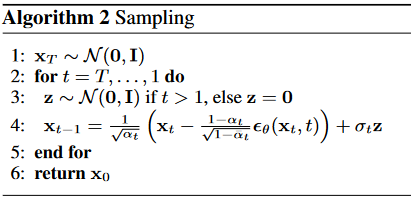
\includegraphics[width=0.45\textwidth]{../images/sample.png}
    \caption{Sample algorithm}
    \label{fig:Samp}
\end{figure}

Figure \ref{fig:Samp} is the sampling algorithm described in the original DDPM
paper. To explain the process at a high level, it first begins with T, where
pure noise is generated, where the trained model is then used to gradually
denoise it. This process is continued until t=0.

\subsection{Simplified Example}

Beyond the forward diffusion process, a majority of the structure for sampling
and the u-net is compiled from various sources.

Unfortunately, due to time constraints, I had to reduce timestep and batch size
as to allow the model to converge faster and ensure it did not get stuck at
some local optima. Naturally, this affected the final output and, with an
already simplified model, had major effects on the output. Regardless, a few
samples managed to generate, as shown below. I also switched between cosine and
linear beta schedules, as I found that linear schedules, although proven to
produce worse results, converged faster.

\begin{figure}[htbp]
    \centering
    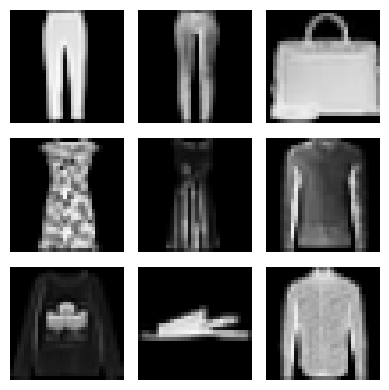
\includegraphics[width=0.45\textwidth]{../images/datasam.png}
    \caption{Sample of FashionMNIST}
    \label{fig:FashionMNIST}
\end{figure}

\begin{figure}[htbp]
    \centering
    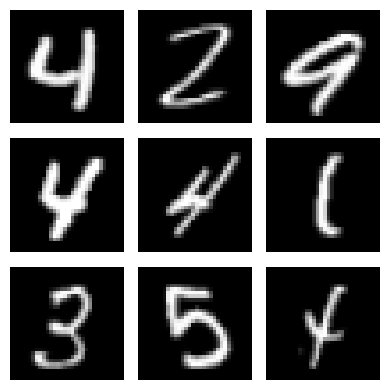
\includegraphics[width=0.45\textwidth]{../images/mnist.png}
    \caption{Sample of MNIST}
    \label{fig:MNIST}
\end{figure}

\begin{figure}[htbp]
    \centering
    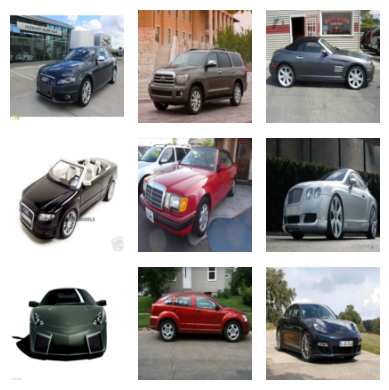
\includegraphics[width=0.45\textwidth]{../images/cars.png}
    \caption{Sample of StandfordCars}
    \label{fig:CARS}
\end{figure}

Figure \ref{fig:FashionMNIST}, \ref{fig:MNIST}, and \ref{fig:CARS} show samples of the datasets
used for the following examples. FashionMNIST consists of 70,000 grayscale images of size 28x28 pixels,
divided into 60,000 images for training and 10,000 images for testing while
MNIST is a dataset of handwritten digits used for training and testing computer
vision models. It consists of 70,000 grayscale images of size 28x28 pixels,
divided into 60,000 images for training and 10,000 images for testing. StandfordCars is a large-scale image recognition dataset that consists of 16,185 images of 196 different car models. The images were collected from various online sources, such as auction websites and dealerships. The samples shown here, are after being processed to fit into tensors for further use, and then reversed back into viewable images, hence why, they are all uniform in size.

\begin{figure}[htbp]
    \centering
    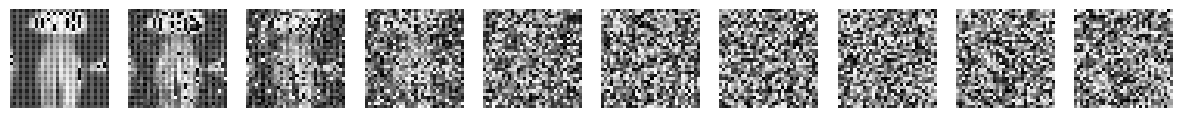
\includegraphics[width=0.45\textwidth]{../images/epoch5.png}
    \caption{FashionMNIST @ epoch 5 | linear schedule}
    \label{fig:epo5}
\end{figure}

\begin{figure}[htbp]
    \centering
    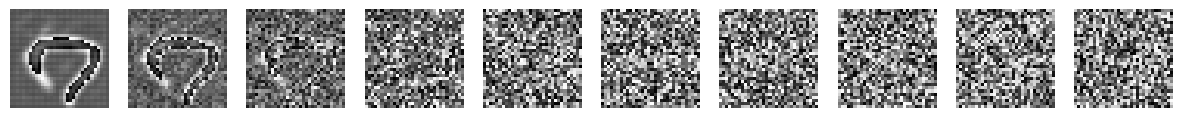
\includegraphics[width=0.45\textwidth]{../images/epoch9-0.png}
    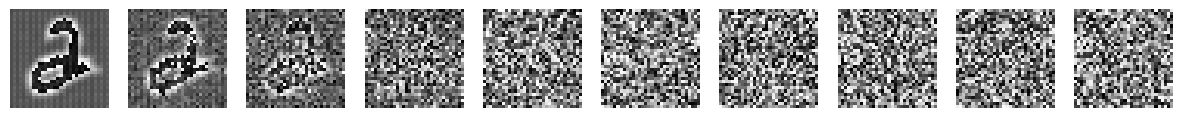
\includegraphics[width=0.45\textwidth]{../images/epoch9-1.png}
    \caption{MNIST @ epoch 9 | linear schedule}
    \label{fig:epo9}
\end{figure}

\begin{figure}[htbp]
    \centering
    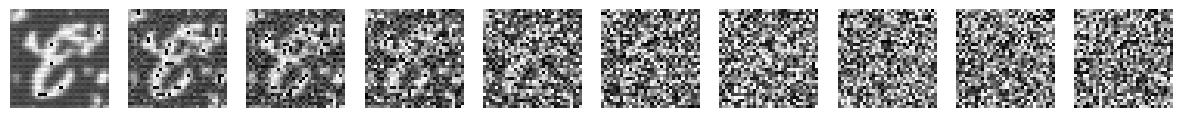
\includegraphics[width=0.45\textwidth]{../images/epoch12.png}
    \caption{MNIST @ epoch 12 | cosine schedule}
    \label{fig:epo12}
\end{figure}

A comparison between the linear, figure \ref{fig:epo9} and cosine schedule,
figure \ref{fig:epo12}, for the MNIST examples exemplifies how the linear
schedule was able to produce a clear attempt at generating a number at epoch 9,
while with cosine at epoch 12, although looks better in terms of color, does
not resemble a number as well. However, various articles and papers also show
how, on the long run, cosine is always the better choice.

Overall, the results of the simplified model are not great, however, this was
to be expected. Regardless, the fact that images are still able to converge
with an un-optimized model on a consumer machine, shows how much DDPMs are
capable of.

\begin{figure}[htbp]
    \centering
    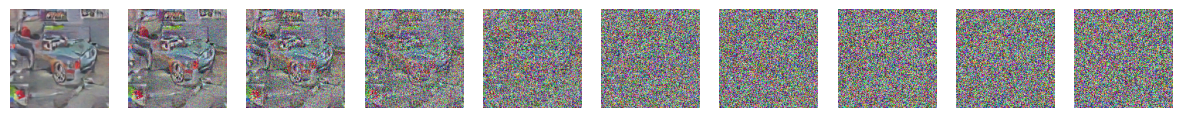
\includegraphics[width=0.45\textwidth]{../images/epoch27-0.png}
    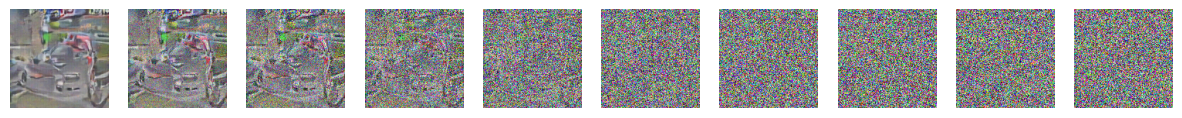
\includegraphics[width=0.45\textwidth]{../images/epoch27-1.png}
    \caption{StandfordCars @ epoch 27 | linear schedule}
    \label{fig:epo27}
\end{figure}

Another quick run using the StandfordCars data set is shown with figure
\ref{fig:epo27}. Due to time, I did have to cut it short, however, it is clear
that some form of image was generating. This examples was using a 128x128 image
to start with, where the previous examples were using only 32. This explains
why at epoch 27 it is still very noisy and scattered.

\begin{figure}[htbp]
    \centering
    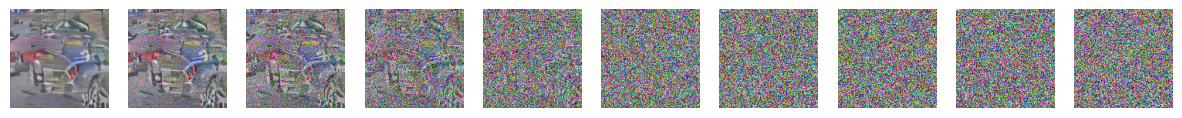
\includegraphics[width=0.45\textwidth]{../images/epoch63.png}
    \caption{StandfordCars @ epoch 63 | linear schedule}
    \label{fig:epo63}
\end{figure}

\begin{figure}[htbp]
    \centering
    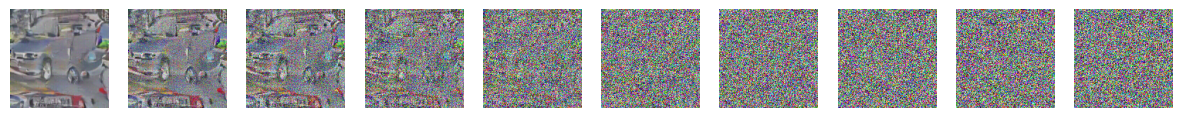
\includegraphics[width=0.45\textwidth]{../images/epoch69.png}
    \caption{StandfordCars @ epoch 69 | linear schedule}
    \label{fig:epo69}
\end{figure}

One final example of the model running the StandfordCars dataset in figure
\ref{fig:epo63} \ref{fig:epo69}, just of an example where running it for longer
does begin to generate more sensible features of a car. However, it still is
not necessarily a single subject, at this point, yet.

The notebook made for this report can be found hosted on github
\href{https://github.com/LeHuman/CS-584-Project/blob/main/simple_ddpm.ipynb}{here}.

\subsection{Conclusion}

Overall, the Denoising Diffusion Probabilistic Model is a very interesting
model, which has recently gained a lot of traction in terms of improvements and
variations. Unfortunately, it is not as well documented or accessible, in terms
of understanding, as something like GAN models, which have been around for
longer. Regardless, I personally have learned a lot with the process of
diffusion models and how they are implemented. Additionally, I have also gained
a more hands on understanding on how applying and using models and techniques
in general is done. Beyond this, DDPMs have already seen incredible
improvements and variations. Some include training for both variance and mean,
versus just mean \cite{nichol2021improved}, including atttention and residual
blocks in the u-net \cite{hugimpl}, and Text to image generation
\cite{saharia2022photorealistic}.

\newpage

\bibliography{refs}
\bibliographystyle{ieeetr}

\end{document}